% !Mode:: "TeX:UTF-8"
%!TEX program  = xelatex

%\documentclass{cumcmthesis}
\documentclass[withoutpreface,bwprint]{cumcmthesis} %去掉封面与编号页
\newcommand{\upcite}[1]{\textsuperscript{\textsuperscript{\cite{#1}}}}
\usepackage{amsmath} 
\usepackage{url}
\title{}
\tihao{A}
\baominghao{4321}
\schoolname{中南大学}
\membera{张震东}
\memberb{杜婷}
\memberc{朱正}
\supervisor{指导老师}
\yearinput{2018}
\monthinput{05}
\dayinput{24}

\begin{document}

 \maketitle
 \begin{abstract}
对于问题一,我们建立了深圳市的人才吸引力评价模型。首先,通过阅读参考文献 、结合马斯洛的需求理论,我们初步给出了17个评价指标(见表一),考虑到指标之间的相关性,对于其中的动态指标,我们收集了近十年的数据,通过聚类分析减少变量,最终确定11个评价指标(见表二)。紧接着,为了达到评价的目的,我们查询了全国范围内的一线城市中指标绝对数值最大的城市,以此为标准,采用不同方法对指标的绝对数值进行修正。再次依据马斯洛的需求层次理论,利用层次分析法获取了指标的权重,最终得到深圳市的得分为76.8。最后,我们找出深圳市关于加大营商环境改革力度的若干措施在人才吸引力方面影响的指标,将其量化,分别求得不同措施下深圳市的得分,并基于此评价深圳市的不同举措对人才吸引力的影响。

对于问题二,我们选取上海和北京为对比城市,运用问题一的人才吸引力评价模型评价对比城市,根据打分权重,并与深圳比较,发现深圳高新技术发展欠佳。其次,我们将人才按行业分类,根据每一个行业的平均工资进行对比分析,得出深圳评价工资为三城市最高。最后建立按行业人才吸引力评价模型,分行业进行评价,并给出了有效提升人才吸引力的可行方案。

针对深圳南山区人才吸引力水平,建立与深圳市人才吸引力评价模型类似的模型,通过分析南山区自身的经济发展特点和其他因素,剔除了环境因素的指标,增加了高新技术发展的指标,并提高房价指标的权重,降低GDP增长率指标的权重;对2014-2016年的人才吸引力进行评估,动态地分析了南山区的人才吸引政策对人才吸引力的影响。

\keywords{人才吸引力\quad  聚类分析\quad   动态分析\quad  层次分析法}
\end{abstract}

%目录
\tableofcontents
\newpage
\section{问题重述}
  在世界各国和全国各地都加大争夺人才的背景下,一个城市要保持其竞争力和创新力,必须要与时俱进但不盲目的调整相关人才吸引政策。深圳市将加大营商环境改革力度作为一项重要工作,以吸引更多优秀人才。
      吸引人才的关键是:符合人才的理想、满足人才的需求和愿望。对于大多数人来说,最先关心的是城市的发展前景,其次是收入,再次是一些环境方面的因素,等等。
\subsection{问题的提出}

本文依次解决如下问题:

(1)量化的评价深圳市的人才吸引力水平,并对深圳市“加大营商环境改革力度若干举措”对人才吸引力的影响做出量化评价。

(2)针对不同人才,深入比较深圳市与其他同类城市在人才吸引力上的优势与不足,并给出有效提升人才吸引力的可行方案。

(3)针对深圳市南山区的经济技术发展特点和相关人才政策,同时考虑人才在各个发展阶段的动态需求,量化评价南山区的人才吸引力水平。


\section{模型的假设}

\begin{itemize}
\item 深圳全市各区在城市绿化、安全指数和自然灾害发生的可能性没有明显的差异,各区的社会保障政策也相同,所以可忽略环境因素指标和社会保障指标;
\item 城镇各行业平均工资与全市各行业平均工资成正比
\end{itemize}


\section{问题分析}

\subsection{问题一分析}
对于该问题,可以利用层次分析法建立深圳市的人才吸引力评价模型。由于所选择的指标之间可能具有相关性,可以利用聚类的方法减少指标。为了达到评价的目的,可查询全国范围内的一线城市中指标绝对数值最大的城市,以此为标准,分别对绝对数值增长与对人才的吸引力呈非线性和线性关系的指标采用不同方法对指标进行修正。结合求得的权重获取得分。最后为了评价深圳市关于加大营商环境改革力度的不同举措对人才吸引力的影响,可以找出深圳市的若干措施在人才吸引力方面影响的指标,将其量化,分别求得不同措施下深圳市的得分。
\subsection{问题二分析}
对于问题二,首先,我们选取对比城市,运用问题一的人才吸引力评价模型评价对比城市,根据打分权重,分析对比城市与深圳的得分排名,找出深圳综合的优势和不足。其次,我们将人才按行业分类,根据每一个行业的平均工资进行对比分析,得出三城市的行业平均工资排名。最后建立按行业人才吸引力评价模型,对行业进行评价,并给出有效提升人才吸引力的可行方案。

\subsection{问题三分析}
在评价深圳南山区人才吸引力水平时我们利用与评价深圳全市人才吸引力水平相似的方法建立评价模型,即通过层次分析法计算各指标的权重,利用无量纲化处理相关指标的数据,最后加权求和得出人才吸引力水平。在本问题确定权重的过程中,我们要重点考察在和深圳市其他地区相比南山区自身的经济发展特点,对相关指标的权重作一定程度的调整,以建立针对南山区人才吸引力水平的模型。


\section{模型建立与求解}
\subsection{人才吸引力评价模型}
\subsubsection{指标选择}
我们阅读了参考文献\upcite{bib:1} ,结合马斯洛的需求理论:人类的需求主要有5个方面:生理需求、安全需求、社交需求、尊重需求和自我实现需求,最终从城市的发展前景、居民生活水平、环境因素、政府激励政策、社会保障五个方面考察城市对人才的吸引力,而对于城市的发展前景,则考虑了近两年深圳市人均GDP增长率、国家的扶持项目数、高等院校数量、世界500强企业的数量等因素,并对部分变量采用取倒数的方法将其全部转化为正向指标,具体见表\ref{tab:zbxq}。

% Table generated by Excel2LaTeX from sheet 'Sheet1'
\linespread{0.5}

\begin{table}[htbp]
  \centering
  \caption{指标选取表格}
    \begin{tabular}{lp{12.665em}p{16.835em}}
    \toprule
    第一级指标 & \multicolumn{1}{l}{第二级指标} & \multicolumn{1}{l}{指标描述} \\
    \midrule
    \multirow{4}[8]{*}{发展前景} & \multicolumn{1}{l}{近五年深圳市人均GDP增长率} & \multicolumn{1}{r}{} \\
\cmidrule{2-3}      & \multicolumn{1}{l}{高等院校数量} & \multicolumn{1}{r}{} \\
\cmidrule{2-3}      & \multicolumn{1}{l}{世界500强企业的数量} & \multicolumn{1}{r}{} \\
\cmidrule{2-3}      & \multicolumn{1}{l}{城市人口迁移情况} & \multicolumn{1}{l}{迁入率-迁出率} \\
    \midrule
    \multirow{3}[6]{*}{生活水平} & \multicolumn{1}{l}{人均年收入} & \multicolumn{1}{r}{} \\
\cmidrule{2-3}      & \multicolumn{1}{l}{住房} & \multicolumn{1}{l}{1/房价} \\
\cmidrule{2-3}      & \multicolumn{1}{l}{平价购买力} & \multicolumn{1}{l}{1/人均年消费性支出} \\
    \midrule
    \multirow{7}[14]{*}{环境因素} & \multicolumn{1}{l}{是否在自然灾害高发带} & \multicolumn{1}{l}{0-1变量} \\
\cmidrule{2-3}      & \multicolumn{1}{l}{空气质量} & \multicolumn{1}{l}{一年中的空气质量优良天数} \\
\cmidrule{2-3}      & \multicolumn{1}{l}{水源质量} & \multicolumn{1}{l}{生活用水达标率} \\
\cmidrule{2-3}      & \multicolumn{1}{l}{城市绿化} & \multicolumn{1}{l}{人均绿化面积} \\
\cmidrule{2-3}      & \multicolumn{1}{l}{交通便捷程度} & \multicolumn{1}{l}{城市内轨道交通线路条数} \\
\cmidrule{2-3}      & \multicolumn{1}{l}{交通道路状况} & \multicolumn{1}{l}{人均拥有道路面积(m2)} \\
\cmidrule{2-3}      & \multicolumn{1}{l}{社会安全指数} & \multicolumn{1}{l}{近五年刑事案件立案数下降率} \\
    \midrule
    政府激励保障 & 人才奖励补贴 & \multicolumn{1}{l}{高层次人才奖励补贴金额} \\
    \midrule
    \multicolumn{1}{l}{\multirow{2}[4]{*}{社会保障}} & 医疗设备 & 每万人拥有的病床数(张) \\
\cmidrule{2-3}      & 社会保险情况 & 平均每人参与社会保险数量 \\
    \bottomrule
    \end{tabular}%
  \label{tab:zbxq}%
\end{table}%



\newpage
其中,是否在自然灾害高发带为0-1变量,即处在自然灾害高发带,则该指标的取值为0,否则为1。接下来,为了动态的反应深圳近几年的经济与社会安全变化情况,我们选择了近五年深圳市人均GDP增长率和近五年刑事案件立案数下降率作为评价指标。
对于已选指标中的随年份变化的动态指标,考虑到一些指标之间可能具有相关性,我们采用聚类分析的方法,对这些指标进行分类,聚类树状图如下:
\begin{figure}[!h]
\centering
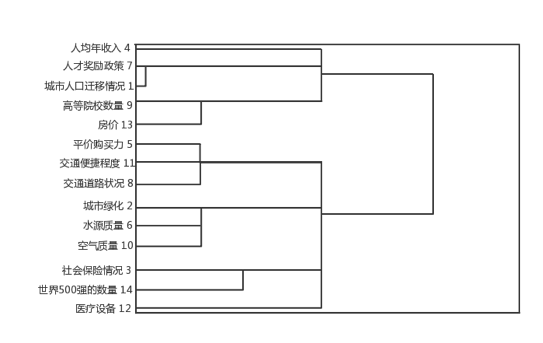
\includegraphics[width=.6\textwidth]{tree.png}
\caption{聚类树状图}
\label{聚类树状图}
\end{figure}

由聚类结果可以看出,表\ref{tab:zbxq}中的部分指标确实与其他指标具有相关性,最终,我们采用了第二次聚类的结果,确定了深圳市人才吸引力评价指标如表\ref{tab:人才吸引力评价指标}所示:
% Table generated by Excel2LaTeX from sheet 'Sheet1'
\begin{table}[htbp]
  \centering
  \caption{人才吸引力评价指标}
    \begin{tabular}{rp{12.665em}p{16.835em}}
    \toprule
    \multicolumn{1}{l}{第一级指标} & \multicolumn{1}{l}{第二级指标} & \multicolumn{1}{l}{指标描述} \\
    \midrule
    \multicolumn{1}{l}{\multirow{3}[6]{*}{发展前景}} & \multicolumn{1}{l}{近五年深圳市人均GDP增长率} & \multicolumn{1}{r}{} \\
\cmidrule{2-3}      & \multicolumn{1}{l}{高等院校数量} & \multicolumn{1}{r}{} \\
\cmidrule{2-3}      & \multicolumn{1}{l}{世界500强企业的数量} & \multicolumn{1}{r}{} \\
    \midrule
    \multicolumn{1}{l}{\multirow{2}[4]{*}{生活水平}} & \multicolumn{1}{l}{人均年收入} & \multicolumn{1}{r}{} \\
\cmidrule{2-3}      & \multicolumn{1}{l}{住房} & \multicolumn{1}{l}{1/平均房价 } \\
    \midrule
    \multicolumn{1}{l}{\multirow{3}[6]{*}{环境因素}} & \multicolumn{1}{l}{是否在自然灾害高发带} & \multicolumn{1}{l}{0-1变量 } \\
\cmidrule{2-3}      & \multicolumn{1}{l}{城市绿化} & \multicolumn{1}{l}{人均绿化面积 } \\
\cmidrule{2-3}      & \multicolumn{1}{l}{社会安全指数} & \multicolumn{1}{l}{(近五年刑事案件立案数下降率)} \\
    \midrule
    \multicolumn{1}{l}{政府激励保障} & 人才奖励补贴 & \multicolumn{1}{l}{高层次人才奖励补贴金额 } \\
    \midrule
    \multicolumn{1}{r}{\multirow{2}[4]{*}{社会保障}} & 医疗设备 & 每万人拥有的病床数(张) \\
\cmidrule{2-3}      & 社会保险情况 & 平均每人参与社会保险数量  \\
    \bottomrule
    \end{tabular}%
  \label{tab:人才吸引力评价指标}%
\end{table}%

\subsubsection{指标的合理量化}
显然,绝对的数据无法达到评价的目的,为此,我们对指标进行了修正:我们分别查询了全国范围内的一线城市中对于表二的指标绝对数值最大的城市,依次为: 北京、北京、北京、北京、沈阳、深圳、东莞、上海、上海、北京、北京。其相应的指标即可认为是最优指标值。
对于表二中的一些指标,当绝对数值增加为k倍时,对人才的吸引力却不是$k$倍,说明这些指标的绝对数值增长与对人才的吸引力呈非线性关系。因此,我们从下面两类对指标进行修正:(设修正后指标数值为$y$,修正前指标数值为$x$,最优指标值为$X_{max}$)

(1)	绝对数值增长与对人才的吸引力呈非线性关系的指标
这类的指标有:人均年收入,
对于这类指标,采用比值的方法不能准确的反映深圳市的相对优秀程度。我们不妨假设非线性指标修正后指标值$y$随修正前数值$x$的变化率为$kx,k>0$。
\par
则有: 
      
\begin{equation}
	\left\{ \begin{array}{l}
\frac{{dy}}{{dx}} = kx\\
y(0) = 0\\
\int_0^{{X_{\max }}} {kxdx = 1} 
\end{array} \right.
\end{equation} 

则可解得k的值,那么    \begin{equation}y = \int_0^x {kxdx} \end{equation} 。


(2)	绝对数值增长与对人才的吸引力呈线性关系的指标
对于这类指标,为了反映在该指标下,深圳市的相对优秀程度,令
   \begin{equation}y = \frac{x}{{{X_{\max }}}}\end{equation} 
这样,所有的指标的取值均在[0,1]之间,最终评价得出的分值也会在[0,1]之间。

\subsubsection{人才吸引力评价模型的建立}
由上文的分析,我们建立了人才吸引力的层次结构如图\ref{tab:人才吸引力的层次结构图}
\begin{figure}[!h]
\centering
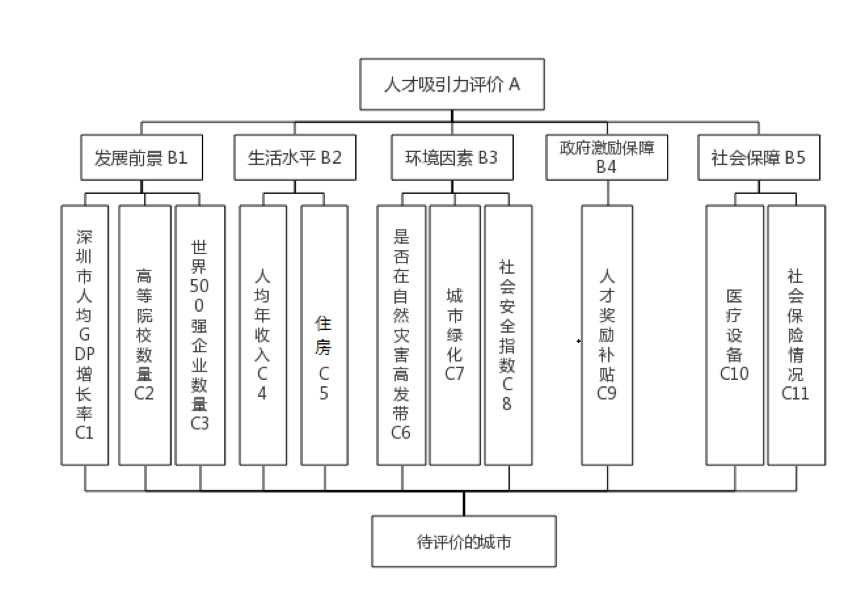
\includegraphics[width=1\textwidth]{appeal.png}
\caption{人才吸引力的层次结构图}
\label{tab:人才吸引力的层次结构图}
\end{figure}
\newpage	
根据马斯洛的需求层次理论,人类的需要按重要性和层次性排成一定次序,从基本的(如住房和饮食)到复杂的(如自我实现)。即位于金字塔上端的指标重要程度会高于金字塔底端的指标,如图\ref{tab:马斯洛需求理论图}所示。
\begin{figure}[!h]
\centering
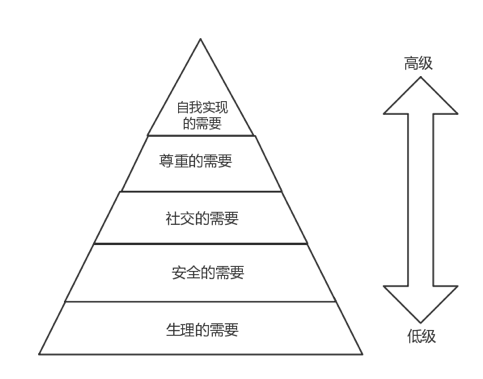
\includegraphics[width=.6\textwidth]{need.png}
\caption{马斯洛需求理论图}
\label{tab:马斯洛需求理论图}
\end{figure}

基于马斯洛的需求理论以及Satty等人给出的1-9尺度,我们可以得出各准则层的成对比较阵。

其中,第一准则层的成对比较阵为
\begin{equation}A = \left( {\begin{array}{*{20}{c}}
1&3&2&5&5\\
{\frac{1}{3}}&1&2&4&3\\
{\frac{1}{2}}&{\frac{1}{2}}&1&2&3\\
{\frac{1}{5}}&{\frac{1}{4}}&{\frac{1}{2}}&1&1\\
{\frac{1}{5}}&{\frac{1}{3}}&{\frac{1}{3}}&1&1
\end{array}} \right)\end{equation}

求得第一准则层对目标层的权向量为: \begin{equation}{w^{(2)}} = (0.4382,0.2433,0.1715,0.0743,0.0727)\end{equation}

一致性指标: \begin{equation}C{I^{(2)}} = 0.0319\end{equation}

一致性比率( RI为随机一致性指标): \begin{equation}C{R^{(2)}} = \frac{{C{I^{(2)}}}}{{R{I^{(2)}}}} = 0.0285 < 0.1\end{equation} 

一致性检验通过。

同样的由第二准则层的成对比较阵(见附录B)可求出第三准则层对第二层的权向量 以及相应的一致性指标 和一致性比率 ,经检验,均通过一致性检验。

由此求出第二准则层对目标层的组合权向量为:  \begin{equation}\begin{split}{w^{(3)}} = &[{w^{(31)}},{w^{(32)}}...{w^{(35)}}] \times {w^{(2)}} \\
=&(0.2548,0.048,0.1354,0.1622,0.0811,0.086,\\&0.0343,0.0686,0.0743,0.0485,0.0242)\end{split}\end{equation}

第二准则层的组合一致性比率为:
 \begin{equation}C{R^{(3)}} = \frac{{[C{I^{(31)}},...,C{I^{(35)}}] \times {w^{(2)}}}}{{[R{I^{(31)}},...,R{I^{(35)}}] \times {w^{(2)}}}} =0.0167<0.1\end{equation}
 
 第二准则层对目标层的组合一致性比率为:
 \begin{equation}C{R^*} = C{R^{(2)}} + C{R^{(3)}} = 0.0452 < 0.1\end{equation}
 组合一致性检验通过,前面的得到的组合权向量 可以作为最终决策的依据,由此得出深圳市关于人才吸引力的得分为0.768。转换为百分制为76.8分。
如果以60分作为及格分数的话,显然深圳市对于人才的吸引力已达及格标准,尽管如此,但由于我们选择的最优数值是全国范围内一线城市中指标最优的城市的数值,因此,从一定程度上讲,深圳是一个比较吸引人才的城市。但从另一方面讲,对于一些权重较大的指标,如高等院校的数量、世界500强企业的数量、住房:,深圳的数值相比于全国一线城市中的最优数值仍有一定的距离,因此,深圳市提高人才吸引力时可以主要从这几方面入手。

\subsubsection{深圳市关于加大营商环境改革力度的若干措施对人才吸引力水平的影响}
深圳市关于加大营商环境改革力度的若干措施中,表\ref{tab:人才吸引力评价指标}中的指标能直接被影响的有
\begin{itemize}
\item 世界500强企业的数量:深圳市不仅计划采取一系列措施以营造更加开放的贸易投资环境,而且还为了营造综合成本适宜的产业发展环境,采取措施降低企业运营成本、降低企业税费负担、优化产业空间资源配置等。而这些措施的最终成果在一定程度上都可由评价模型中的指标:世界500强企业的数量来反映。
\item 住房:实施更优惠的人才住房政策显然能够降低人才的购房负担。
\item 城市绿化
\item 加大人才奖励力度。
\end{itemize}

除了上述指标,举措中涉及的其他指标在1.1的聚类分析中发现与其他指标有相关性联系,故这里我们不再重复考虑。
由1.1的评价模型得知,上述四个指标的权重分别是0.1354、0.0811、0.0343、0.0743.
为了定量的评价深圳市的一系列举措,考虑到通知中提到的举措的施行力度与广度,以及原有指标数值的基数大小,我们不妨假设自深圳市实行这些举措一段时间之后,四个指标的绝对数值分别增加了原来的50\%、10\%、5\%、10\%,那么相应的修正数值也改变同等比例。在1.1的人才吸引力评价模型得出的分数的基础上,分别作出相应的改变后,得到的新的分数为:
 79.44、78.14、79.39、83.01.显然,深圳市的一系列举措都在一定程度上有效增加了对人才的吸引力,其中以加大人才奖励力度的效果最为明显,其次是对企业的扶持也起到了正向作用。

\subsection{按行业分人才吸引力对比分析}
根据国家统计局数据,我们选取北京、上海两个一线城市作为对比城市。
\subsubsection{数据处理}
由于由于北京统计与上海统计对于平均工资的统计范围不同(如下):北京采用的是城镇单位在岗职工平均工资(式\ref{tab:城镇单位在岗职工平均工资} ),上海、深圳采用的是职工平均工资(式\ref{tab:职工平均工资})。因此必须对两个平均工资的数据进行处理,以比较两地的平均工资问题。


\begin{equation}
	w_{\mbox{\tiny 城镇单位在岗职工平均工资}}=\frac{t_{\mbox{\tiny 报告期城镇单位在岗职工工资总额}}}{p_{\mbox{\tiny 报告期城镇单位在岗职工平均人数} }}
	\label{tab:城镇单位在岗职工平均工资}
\end{equation}

	
\begin{small}{\textbf{注}\,单位从业人员工资总额:指各单位在一定时期内直接支付给本单位全部从业人员的工资总额。包括在岗 职工的工资总额和其他从业人员的工资总额两部分 
}
\end{small}

\begin{equation}
	w_{\mbox{\tiny 职工平均工资}}=\frac{t_{\mbox{\tiny 报告期职工工资总额}}}{p_{\mbox{\tiny 报告期职工平均人数} }}
	\label{tab:职工平均工资}
\end{equation}

	
	
\begin{small}{
\textbf{注}\,在岗职工工资总额:指各单位在一定时期内直接支付给本单位在岗职工的工资总额。}
\end{small}

为了统一三地平均工资的量度,根据本题研究主要方向为全地区人才吸引力情况衡量,因此我们统一采用全地区平均工资标准,从而我们仅需对北京数据进行处理。

对北京的职工平均工资处理方法如下:

根据北京城镇各行业平均工资与北京全市各行业平均工资成正比的假设,首先我们求出城镇单位在岗职工平均工资与职工平均工资的比例系数$\rho$,
\begin{equation}
	\rho=\frac{w_{\mbox{\tiny 城镇单位在岗职工平均工资}}}{w_{\mbox{\tiny 职工平均工资}} }	
\end{equation}

而后将比例系数与北京城镇城镇单位在岗职工平均工资相除,得到预估北京职工平均工资
\begin{equation}
\overline{w}_{\mbox{\tiny 预估职工平均工资}}=\frac{w_{\mbox{\tiny 城镇单位在岗职工平均工资}}}{\rho}
\label{tab:预估职工平均工资}	
\end{equation}


因为北京市职工平均工资为92477元\upcite{bib:2},北京城镇平均工资为122749元\upcite{bib:3},根据公式得出比例系数$\rho=1.33$。根据北京市统计局北京城镇分行业平均工资数据(附录C),以及公式\ref{tab:预估职工平均工资},可以得到北京职工分行业预估平均工资数据表:
% Table generated by Excel2LaTeX from sheet 'Sheet1'
\begin{table}[htbp]
  \centering
  \caption{北京职工分行业预估平均工资数据表}
    \begin{tabular}{|l|r|r|r|r|}
    \toprule
    项目 & \multicolumn{1}{l|}{北京平均工资} & \multicolumn{1}{l|}{国有单位} & \multicolumn{1}{l|}{集体单位} & \multicolumn{1}{l|}{其他单位} \\
    \midrule
    合计 & 92477  & 129542  & 59507  & 122096  \\
    \midrule
    农、林、牧、渔业 & 39421  & 83330  & 39092  & 48476  \\
    \midrule
    采矿业 & 68666  &   & 42131  & 91588  \\
    \midrule
    制造业 & 72712  & 114749  & 47360  & 96566  \\
    \midrule
    电力、热力、燃气及水生产和供应业 & 102807  & 166944  & 50607  & 129583  \\
    \midrule
    建筑业 & 68785  & 93557  & 74944  & 91752  \\
    \midrule
    批发和零售业 & 77161  & 138352  & 54145  & 101511  \\
    \midrule
    交通运输、仓储和邮政业 & 68287  & 95877  & 33730  & 90172  \\
    \midrule
    住宿和餐饮业 & 43967  & 63550  & 51367  & 57717  \\
    \midrule
    信息传输、软件和信息技术服务业 & 127845  & 165516  & 57042  & 169848  \\
    \midrule
    金融业 & 217455  & 240719  & 82743  & 289937  \\
    \midrule
    房地产业 & 71431  & 93426  & 53306  & 96808  \\
    \midrule
    租赁和商务服务业 & 86679  & 96159  & 47277  & 123521  \\
    \midrule
    科学研究和技术服务业 & 108729  & 166611  & 100547  & 134302  \\
    \midrule
    水利、环境和公共设施管理业 & 59485  & 81843  & 39104  & 77247  \\
    \midrule
    居民服务、修理和其他服务业 & 39822  & 61513  & 39246  & 52491  \\
    \midrule
    教育 & 94369  & 137922  & 76809  & 81119  \\
    \midrule
    卫生和社会工作 & 114668  & 168987  & 95272  & 84797  \\
    \midrule
    文化、体育和娱乐业 & 106827  & 161428  & 50445  & 117363  \\
    \midrule
    公共管理、社会保障和社会组织 & 81417  & 111904  & 73126  & 61739  \\
    \bottomrule
    \end{tabular}%
  \label{tab:北京职工分行业预估平均工资数据表}%
\end{table}%


\newpage	
\subsubsection{北京、上海、深圳人才吸引力评价及对比}
运用第一问的人才吸引力评价模型,根据国家统计局数据\upcite{bib:2},对改进过的北京数据和上海两个城市进行综合评价:

% Table generated by Excel2LaTeX from sheet 'Sheet1'
\begin{table}[htbp]\small
  \centering
  \caption{北京、上海、深圳综合得分}
    \begin{tabular}{l|l|llllll}
      & \textbf{最优指标数值} & \textbf{北京} & \textbf{绝对数值} & \textbf{上海} & \textbf{绝对数值} & \textbf{深圳} & \textbf{绝对数值} \\
    \midrule
    \textbf{近五年人均GDP增长率} & 0.087214 & 1 & 0.08721 & 0.96 & 0.084 & 0.91 & 0.07937 \\
    \textbf{高等院校数量} & 91 & 1 & 91 & 0.703 & 64 & 0.13 & 12 \\
    \textbf{500强企业} & 48 & 1 & 48 & 0.9375 & 45 & 0.125 & 6 \\
    \textbf{可支配收入} & 57275 & 1 & 57275 & 0.948 & 51179 & 0.85 & 48695 \\
    \textbf{1/房价} & 8018.25 & 0.158 & 50734 & 0.148 & 54305 & 0.15 & 51119 \\
    \textbf{是否在自然灾害高发带} & 1 & 1 & 1 & 1 & 1 & 1 & 1 \\
    \textbf{人均绿地面积} & 22.91 & 0.489 & 11.2 & 0.358 & 8.2 & 0.72 & 16.5 \\
    \textbf{刑事案件立案数下降率} & 3.80\% & 1 & 3.80\% & 1 & 3.80\% & 0.816 & 3.10\% \\
    \textbf{高层次人才奖励补贴金额(万元)} & 1657.89 & 0.91 & 1508.68 & 1 & 1657.9 & 0.76 & 1260 \\
    \textbf{每万人拥有病床数} & 46.43 & 1 & 46.43 & 0.991 & 46 & 0.69 & 32 \\
    \textbf{平均每人参与社会保险数量} & 5.095 & 1 & 5.095 & 0.956 & 4.869 & 0.91 & 4.63671 \\
    \midrule
    \textbf{得分} &   & 0.9054 &   & 0.8661 &   & 0.7680 &  \\
    \end{tabular}%
  \label{tab:北京、上海、深圳综合得分}%
\end{table}%
得出排名依次为北京、上海、深圳,深圳由于500强企业以及高等院校数量过少导致得分偏低。

\subsubsection{北京、上海、深圳各行业职工平均工资对比}
根据国家统计局数据,可以得到这三个城市的各行业职工平均工资对比柱状图(图4)

	


\begin{figure}[!h]
\centering
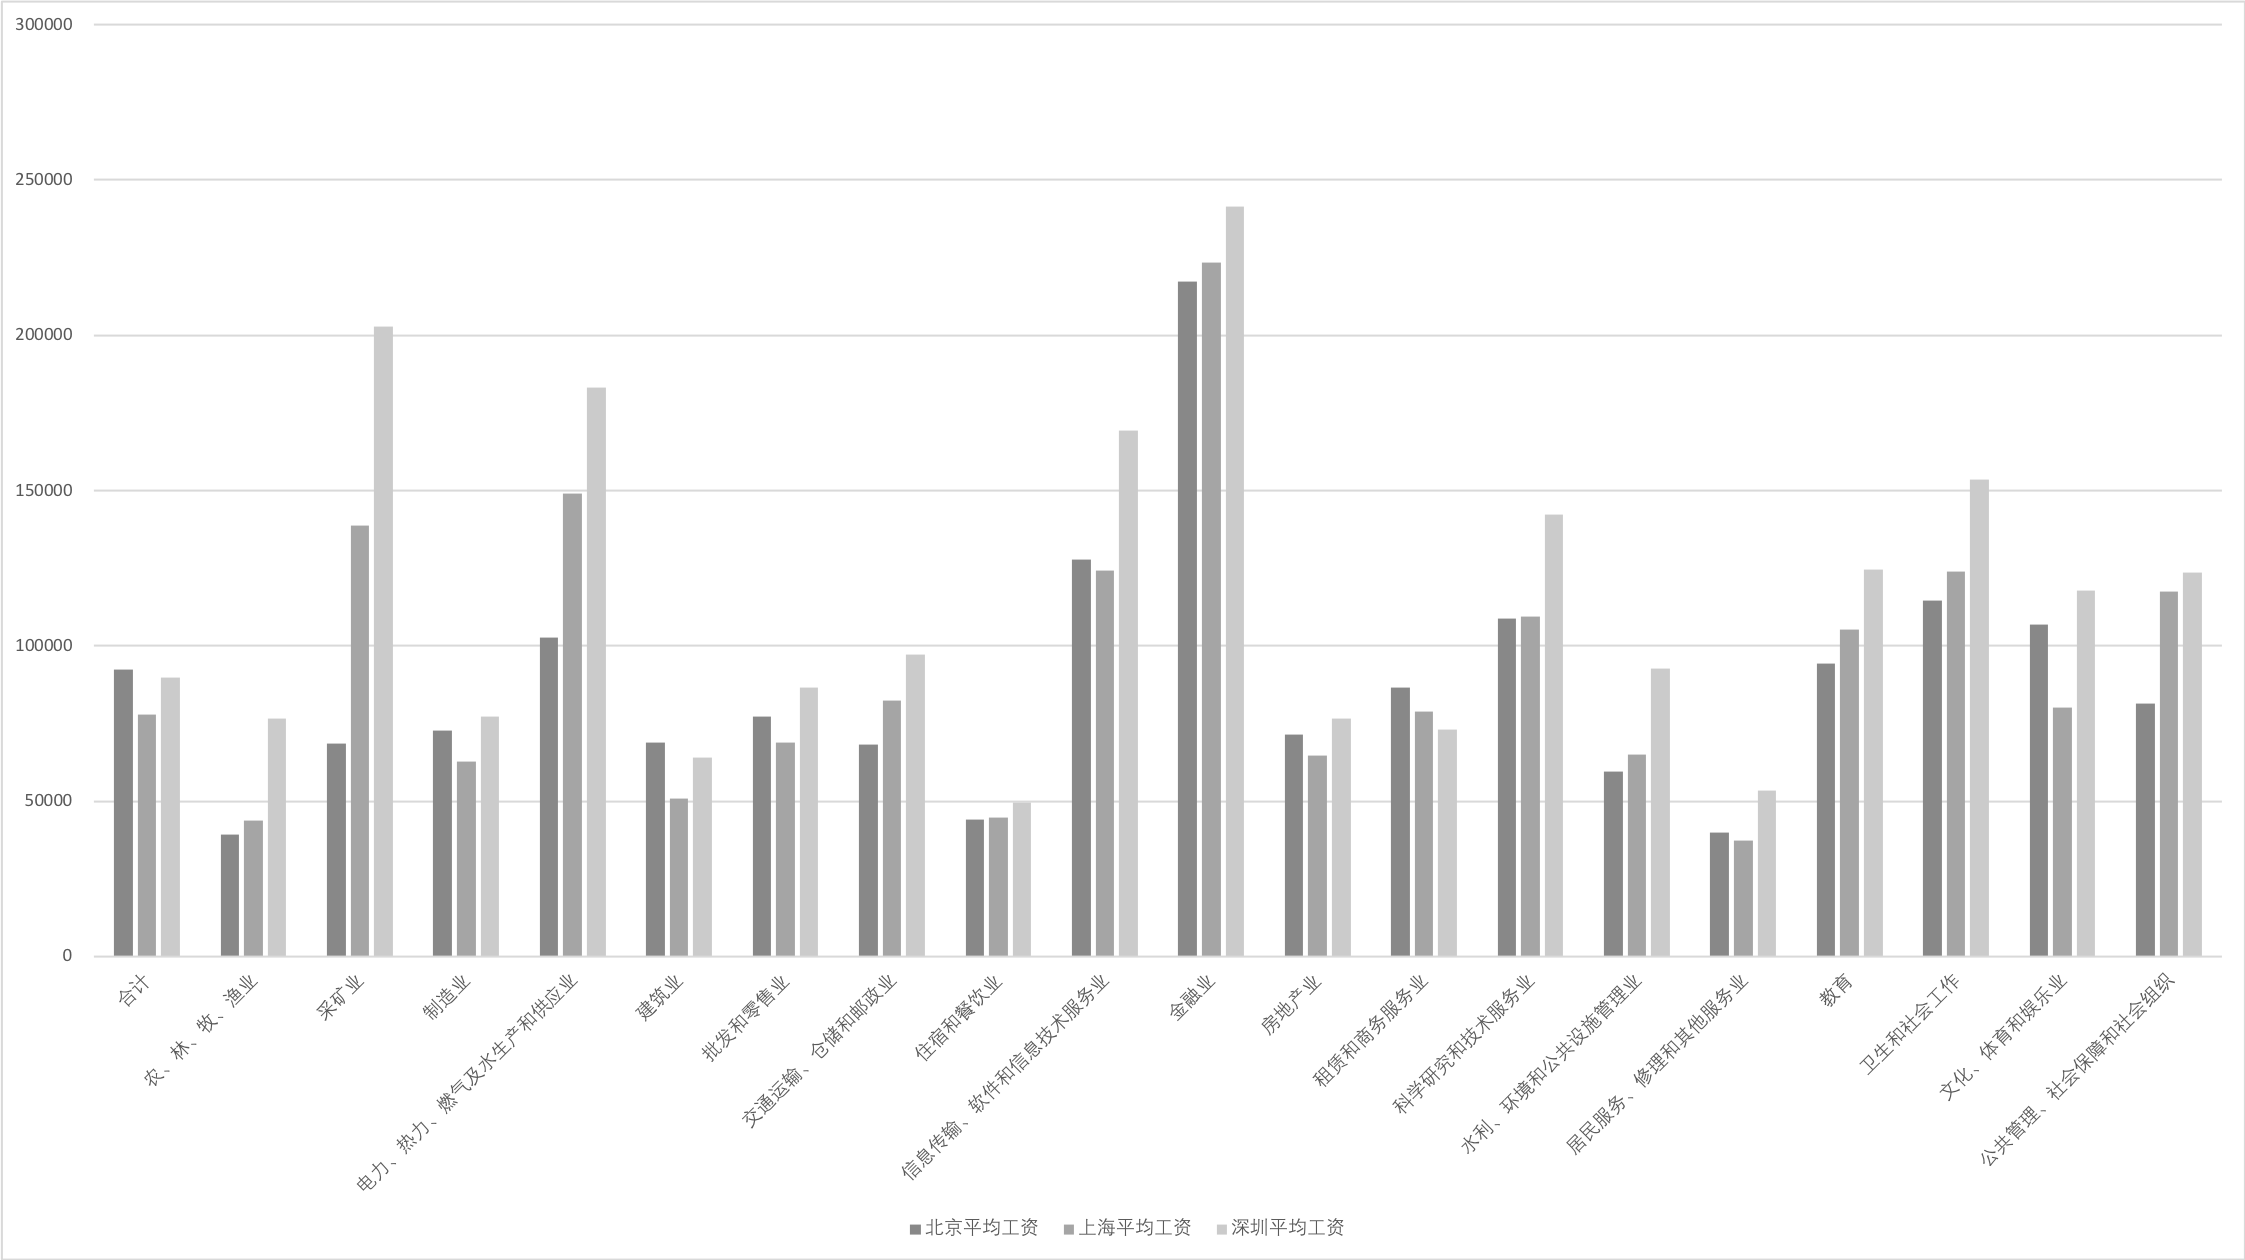
\includegraphics[width=1\textwidth]{wages.png}
\caption{北京、上海、深圳各行业职工平均工资对比柱状图
}
\label{tab:北京、上海、深圳各行业职工平均工资对比柱状图
}
\end{figure}

可以发现,金融业以及信息传输、软件和信息技术服务业的平均工资是最高的,深圳的平均工资高于其他两个城市,深圳的工资表现在这三者之间表现最佳。
\subsubsection{北京、上海、深圳各行业职工综合评价对比}
为了更好的反映各行业的发展优势和不足,我们在第一问的基础上对原有模型进行了修改,将平均工资指标修改为各行业工资指标,综合评价各行业在北京、上海、深圳三个城市的发展状况。根据中国统计局数据\upcite{bib:2},我们得出了各行业在北京、上海、深圳三个城市的打分,打分表如表\ref{tab:北京、上海、深圳各行业职工综合评价}。
% Table generated by Excel2LaTeX from sheet 'Sheet1'
\begin{table}[htbp]\small
  \centering
  \caption{北京、上海、深圳各行业职工综合评价}
    \begin{tabular}{l|rrr|rl}
      & \multicolumn{1}{l}{北京行业得分} & \multicolumn{1}{l}{上海行业得分} & \multicolumn{1}{l|}{深圳行业得分} & \multicolumn{1}{l}{最大得分} & 最大得分城市 \\
    \midrule
    农、林、牧、渔业 & 0.8289 & 0.8053 & 0.7906 & 0.8289 & 北京 \\
    采矿业 & 0.8002 & 0.8232 & 0.7906 & 0.8232 & 上海 \\
    制造业 & 0.8978 & 0.8442 & 0.7906 & 0.8978 & 北京 \\
    电力、热力、燃气及水生产和供应业 & 0.8364 & 0.8442 & 0.7906 & 0.8442 & 上海 \\
    建筑业 & 0.9075 & 0.832 & 0.7796 & 0.9075 & 北京 \\
    批发和零售业 & 0.89 & 0.8417 & 0.7906 & 0.89 & 北京 \\
    交通运输、仓储和邮政业 & 0.8591 & 0.8499 & 0.7906 & 0.8591 & 北京 \\
    住宿和餐饮业 & 0.8891 & 0.8584 & 0.7906 & 0.8891 & 北京 \\
    信息传输、软件和信息技术服务业 & 0.8678 & 0.8315 & 0.7906 & 0.8678 & 北京 \\
    金融业 & 0.8915 & 0.8624 & 0.7906 & 0.8915 & 北京 \\
    房地产业 & 0.8968 & 0.8492 & 0.7906 & 0.8968 & 北京 \\
    租赁和商务服务业 & 0.9075 & 0.86 & 0.7651 & 0.9075 & 北京 \\
    科学研究、技术服务业 & 0.8692 & 0.8371 & 0.7906 & 0.8692 & 北京 \\
    水利、环境和公共设施管理业 & 0.8493 & 0.8258 & 0.7906 & 0.8493 & 北京 \\
    居民服务、修理和其他服务业 & 0.8661 & 0.8254 & 0.7906 & 0.8661 & 北京 \\
    教育 & 0.8683 & 0.8493 & 0.7906 & 0.8683 & 北京 \\
    卫生和社会工作 & 0.8663 & 0.8431 & 0.7906 & 0.8663 & 北京 \\
    文化、体育和娱乐业 & 0.8925 & 0.8226 & 0.7906 & 0.8925 & 北京 \\
    公共管理、社会保障和社会组织 & 0.8521 & 0.8662 & 0.7906 & 0.8662 & 上海 \\
    \end{tabular}%
  \label{tab:北京、上海、深圳各行业职工综合评价}%
\end{table}%

根据最大得分城市排名,我们发现深圳市较为落后。由评价的权重和具体数据来看,深圳市高新技术发展欠佳,国家级高新技术企业数量和专利授权数相比于北京和上海还有很大差距。
\newpage
\subsubsection{深圳人才吸引改进方案}

\begin{itemize}
\item 吸引企业,增加世界500强企业的数量
\item 发展教育,吸引人才前来求学,增加人才流入,发展高新技术
\item 实施更优惠的人才住房政策显然能够降低人才的购房负担
\item 扩大城市绿化面积
\item 加大人才奖励力度
\end{itemize}




\subsection{深圳南山区人才吸引力水平评价模型}
在评价深圳南山区人才吸引力水平时我们利用与评价深圳全市人才吸引力水平相似的方法建立评价模型,即通过层次分析法计算各指标的权重,利用无量纲化处理相关指标的数据,最后加权求和得出人才吸引力水平。在本问题确定权重的过程中,我们要重点考察在和深圳市其他地区相比南山区自身的经济发展特点,对相关指标的权重作一定程度的调整,以建立针对南山区人才吸引力水平的模型。

考虑到南山区和深圳市其他区在环境、经济发展特点等方面的异同,通过分析南山区统计公报以及其他实际情况,我们得出以下结论并做出一些合理的假设:

(1)	深圳全市各区在城市绿化、安全指数和自然灾害发生的可能性没有明显的差异,各区的社会保障政策也相同,所以可忽略环境因素指标和社会保障指标。

(2)	通过分析南山区近年本地生产总值及增长速度(如图\ref{tab:2011-2016年南山区生产总值及增长速度图}所示),我们发现2014年至2016年,南山区生产总值的增长速度保持平稳,且较2011年至2013年相比有下降趋势,因此生产总值的增长对于人才吸引的作用在减小,因此应降低生产总值指标的权重。
\begin{figure}[!h]
\centering
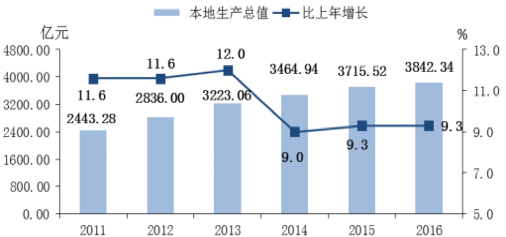
\includegraphics[width=.8\textwidth]{gdp.png}
\caption{2011-2016年南山区生产总值及增长速度图}
\label{tab:2011-2016年南山区生产总值及增长速度图}
\end{figure}
 
      

(3)	由2016年南山区统计公报,南山区工业增长速度逐年下降(如图\ref{tab:2016年南山区工业增加值及增长速度图}所示),第三产业中战略新兴产业增加值 2570.35 亿元,比上年增长13.9\%,占地区生产总值比重达 66.9\%。2016年全区有国家级高新技术企业 2223 家,占全市总量的 27.7\%; 全年专利申请量达 47768 件,比上年增长 52.6\%;专利授权量 20374件,比上年增长 5.4\%。说明南山区已经进行产业转型,第二产业的比重下降,第三产业比重上升;南山区的经济发展以科学技术为重,并通过优良的科研技术环境吸引人才。因此应增加高新技术发展的指标(高新企业数量)并尽可能提高该指标的权重。
\begin{figure}[!h]
\centering
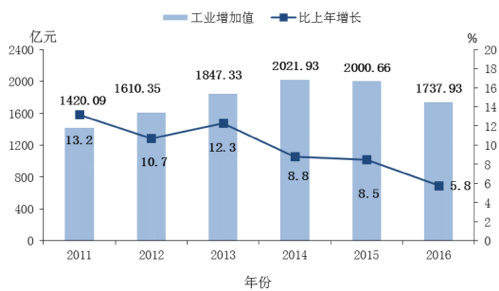
\includegraphics[width=.8\textwidth]{industry.png}
\caption{2016年南山区工业增加值及增长速度图}
\label{tab:2016年南山区工业增加值及增长速度图}
\end{figure}
 
  

(4)	南山区房价和增长速度常年位于全市第一位,房价的变化对于人才吸引的影响必定会大于其他各区,所以房价指标的权重应提高。

根据以上假设,我们确定了南山区人才吸引力评价指标:
\begin{figure}[!h]
\centering
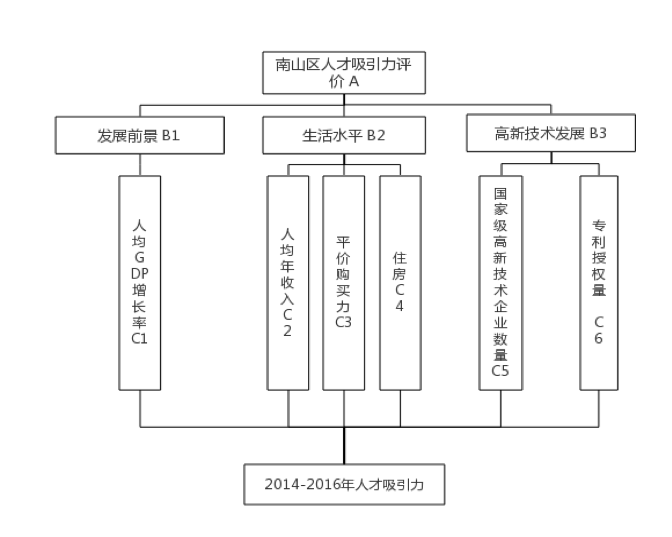
\includegraphics[width=.7\textwidth]{appeal2.png}
\caption{南山区人才吸引力评价指标图}
\label{tab:南山区人才吸引力评价指标图}
\end{figure}
 
\newpage  
并确定了各层次的成对比较矩阵如下:
     
\begin{equation}{B_1} = \left( {\begin{array}{*{20}{c}}
1&{1/3}&{1/5}\\
3&1&{1/3}\\
5&3&1
\end{array}} \right)\end{equation}    
   
\begin{equation}{C_2} = \left( {\begin{array}{*{20}{c}}
1&1&{1/5}\\
1&1&{1/5}\\
5&5&1
\end{array}} \right)\end{equation}    
  
\begin{equation}{C_3} = \left( {\begin{array}{*{20}{c}}
1&3\\
{1/3}&1
\end{array}} \right)\end{equation} 

最终各个指标的权重如下表所示:


% Table generated by Excel2LaTeX from sheet 'Sheet1'
\begin{table}[htbp]
  \centering
  \caption{南山区人才吸引力评价各指标权重表}
    \begin{tabular}{lp{12.665em}l}
    \toprule
    \multicolumn{1}{p{6em}}{一级指标} & 二级指标 & \multicolumn{1}{p{5.25em}}{权重} \\
    \midrule
    \multicolumn{1}{p{6em}}{发展前景} & GDP增长率 & 0.1047 \\
    \multicolumn{1}{l}{\multirow{3}[0]{*}{生活水平}} & 可支配收入 & 0.0369 \\
      & 消费性支出 & 0.0369 \\
      & 房价 & 0.1845 \\
    \multicolumn{1}{l}{\multirow{2}[1]{*}{高新技术发展}} & 国家级高新技术企业数量 & 0.4777 \\
      & 专利授权数 & 0.1592 \\
    \bottomrule
    \end{tabular}%
  \label{tab:南山区人才吸引力评价各指标权重表}%
\end{table}%
   
考虑人才吸引力在时间上的动态变化,我们选取2014—2016年这3年各指标的数据进行无量纲化处理来进行评价。由于模型仅考虑各指标随着时间的推移发生变化,并没有考虑与其他区的比较,所以可以假设数值的增长与人才吸引力呈线性关系,即:对于正向指标,令  $y = \frac{x}{{{x_{\max }}}}$,对于负向指标,  $y = \frac{{{x_{\min }}}}{x}$,其中 ${x_{\max }},{x_{\min }}$分别为各指标在3年间的最大值和最小值。以 作为各指标的数值,这样所有的指标的取值均在[0,1]之间,最终评价得出的分值也会在[0,1]之间。

经过以上处理,我们得到南山区2014年-2016年人才吸引力水平(转换为百分制)
% Table generated by Excel2LaTeX from sheet 'Sheet1'
\begin{table}[htbp]
  \centering
  \caption{南山区2014年-2016年人才吸引力指数表}
    \begin{tabular}{|p{7.335em}|c|c|c|}
    \toprule
    年份 & 2014 & 2015 & 2016 \\
    \midrule
    人才吸引力指数 & 78.08 & 78.71 & 90.27 \\
    \bottomrule
    \end{tabular}%
  \label{tab:南山区2014年-2016年人才吸引力指数表}%
\end{table}%

  
我们可以看出南山区在2016年人才吸引力指数出现大幅度增长。实际上,在2016年,南山区开始推行“领航计划”,对于各类人才给予住房、医疗、学术研究、社会保障上的补贴,这对于人才吸引起到至关重要的作用。上述结果也很好地证明了人才吸引政策的有效性。

\section{模型评价}
\textbf{优点:}
	\begin{itemize}
\item 运用层次分析法确定权重时,我们结合了马斯洛的需求金字塔建立成对比较阵,避免了主观因素的影响
\item 为了达到评价的目的,我们没有使用指标的绝对数值,而是查询全国的一线城市中所有指标的最优数值,利用它们对不同类别的指标数值进行修正。

\end{itemize}

	

\textbf{不足:}
	

\begin{itemize}
\item 在人才吸引力评价模型中,考虑到指标之间的相关性,我们采用聚类的方法对指标分类,对第二次聚类结果,从每类中选择与其他指标性关性最强的一个代表这一类指标,在这个过程中会有误差的存在。


\end{itemize}







\newpage
%参考文献
\begin{thebibliography}{9}%宽度9
 \bibitem{bib:1} 李华. 西安市人才吸引力评价及比较研究[D].西安理工大学,2010.
 \bibitem{bib:4}北京市人力资源和社会保障局, 北京市统计局. 《关于公布2016年度北京市职工平均工资的通知》[N]. 北京市统计快讯, 2016
 \bibitem{bib:2}中国统计局. 《中国统计年鉴—2017》[DB/OL].http://www.stats.gov.cn/tjsj/ndsj/2017/indexch.htm, 2017.05.14
 \bibitem{bib:3}北京统计局. 《北京统计年鉴—2017》[DB/OL]. http://www.bjstats.gov.cn/nj/main/2017-tjnj/zk/indexce.htm, 2017.05.17
  \bibitem{bib:5}张瀚月. 美国城市舒适性评价及其对人才吸引力的影响[D].华东师范大学,2017.
 \bibitem{bib:6} 深圳统计年鉴2017.深圳统计局,2017
  \bibitem{bib:7}深圳市南山区 2016 年国民经济和社会发展统计公报
 



\end{thebibliography} 

\newpage
%附录
\appendix
\section{南山区人才吸引指标原始数据}
% Table generated by Excel2LaTeX from sheet 'Sheet1'
\begin{table}[htbp]
  \centering
    \begin{tabular}{|c|c|c|c|}
    \toprule
      & 2014年 & 2015年 & 2016年 \\
    \midrule
    GDP增长率 & 9.00\% & 9.30\% & 9.30\% \\
    \midrule
    可支配收入 & 53068 & 58180 & 63097 \\
    \midrule
    消费性支出 & 35771 & 41198 & 46925 \\
    \midrule
    房价 & 34163 & 55998 & 65605 \\
    \midrule
    国家级高新企业数量 & 1463 & 1641 & 2223 \\
    \midrule
    专利授权量 & 14415 & 19339 & 20374 \\
    \bottomrule
    \end{tabular}%
  \label{tab:addlabel}%
\end{table}%
 \section{深圳市人才吸引力评价模型第二准则层的成对比较阵}
\begin{equation}{C_1} = \left( {\begin{array}{*{20}{c}}
1&5&2\\
{\frac{1}{5}}&1&{\frac{1}{3}}\\
{\frac{1}{2}}&3&1
\end{array}} \right)\end{equation}                  
\begin{equation}{C_2} = {C_5} = \left( {\begin{array}{*{20}{c}}
1&2\\
{\frac{1}{2}}&1
\end{array}} \right)\end{equation}

\newpage
\section{北京市统计局北京城镇分行业平均工资数据}
% Table generated by Excel2LaTeX from sheet 'Sheet2'
\begin{table}[htbp]
  \centering

    \begin{tabular}{|l|l|l|l|l|}
    \toprule
    项目 & 平均工资 & 国有单位 & 集体单位 & 其他单位 \\
    \midrule
    合计 & 122749 & 129542 & 59507 & 122096 \\
    \midrule
    农、林、牧、渔业 & 52325 & 83330 & 39092 & 48476 \\
    \midrule
    \#农、林、牧、渔服务业 & 54523 & 87573 & 46352 & 35209 \\
    \midrule
    采矿业 & 91144 &   & 42131 & 91588 \\
    \midrule
    制造业 & 96514 & 114749 & 47360 & 96566 \\
    \midrule
    电力、热力、燃气及水生产和供应业 & 136460 & 166944 & 50607 & 129583 \\
    \midrule
    建筑业 & 91301 & 93557 & 74944 & 91752 \\
    \midrule
    批发和零售业 & 102420 & 138352 & 54145 & 101511 \\
    \midrule
    交通运输、仓储和邮政业 & 90640 & 95877 & 33730 & 90172 \\
    \midrule
    住宿和餐饮业 & 58359 & 63550 & 51367 & 57717 \\
    \midrule
    信息传输、软件和信息技术服务业 & 169695 & 165516 & 57042 & 169848 \\
    \midrule
    金融业 & 288638 & 240719 & 82743 & 289937 \\
    \midrule
    房地产业 & 94814 & 93426 & 53306 & 96808 \\
    \midrule
    租赁和商务服务业 & 115053 & 96159 & 47277 & 123521 \\
    \midrule
    科学研究和技术服务业 & 144321 & 166611 & 100547 & 134302 \\
    \midrule
    水利、环境和公共设施管理业 & 78957 & 81843 & 39104 & 77247 \\
    \midrule
    居民服务、修理和其他服务业 & 52858 & 61513 & 39246 & 52491 \\
    \midrule
    教育 & 125260 & 137922 & 76809 & 81119 \\
    \midrule
    卫生和社会工作 & 152204 & 168987 & 95272 & 84797 \\
    \midrule
    文化、体育和娱乐业 & 141797 & 161428 & 50445 & 117363 \\
    \midrule
    公共管理、社会保障和社会组织 & 108069 & 111904 & 73126 & 61739 \\
    \bottomrule
    \end{tabular}%
\label{tab:北京市统计局北京城镇分行业平均工资数据}%
\end{table}%

\end{document} 